\section{Auswertung}
\label{sec:Auswertung}
Im folgendem wird $D$ durch $D=\frac{F}{\Delta x}$ berechnet.
\begin{table}
    \centering
    \caption{Messdaten.}
    \begin{tblr}{colspec={c c c}}
        \toprule
        $\text{Auslenkung }\Delta x \; [cm]$ & $\text{Kraft }F \; [N]$ & $\text{Federkonstante }D \; [\frac {N}{cm}]$ \\
        \midrule
        5 &0.15 &0.03\\
        15 &0.44 &0.0293\\
        10 &0.29& 0.029\\
        25 &0.74& 0.0296\\
        20 &0.59& 0.0295\\
        35 &1.04& 0.0297\\
        30 &0.89& 0.0297\\
        45 &1.34& 0.0298\\
        40 &1.19& 0.0298\\
        50 &1.49& 0.0298\\
        \bottomrule
    \end{tblr}
\end{table}
%
Der Mittelwert von $D$ ist $0.0296 \; [\frac{N}{cm}]$.\\
Die Steigung der Regressionsgerade, welche den Wert von $D$ entspricht, ist $0.0299 \; [\frac{N}{cm}]$.
%
\begin{figure}
    \centering
    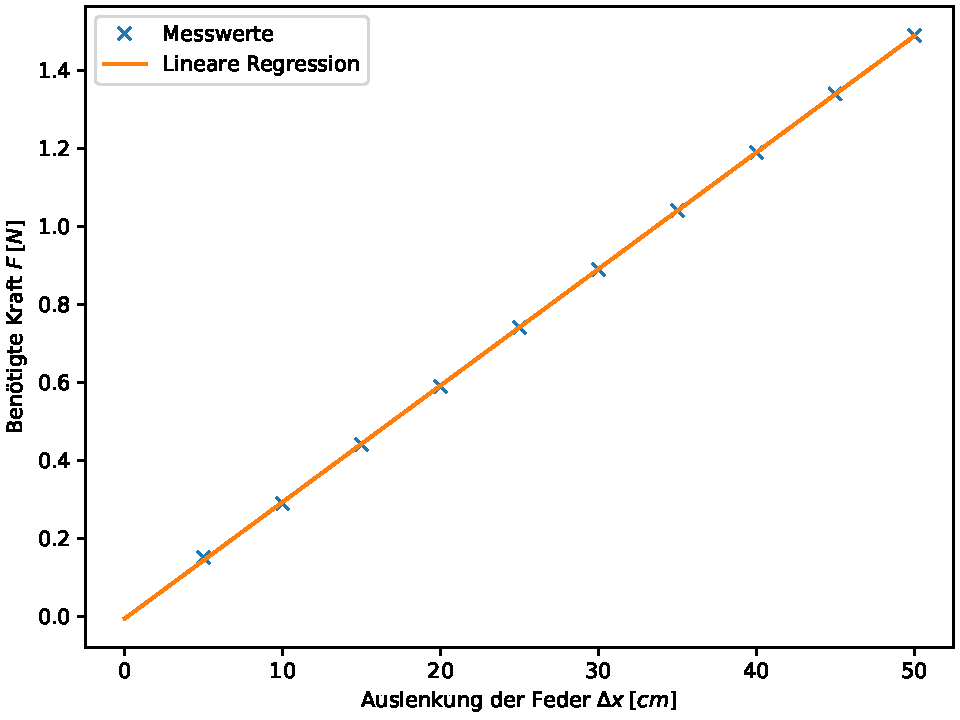
\includegraphics{plot.pdf}
\end{figure}
